%%%% Document type  %%%%
\documentclass[preprint,12pt,fleqn]{article}
 \usepackage{ragged2e}
\usepackage{authblk}  % Package for author affiliations
% \usepackage{nopageno} % no page numbers
\usepackage{placeins} % \FloatBarrier

\usepackage[most]{tcolorbox}
\newtcolorbox[auto counter,number within=chapter]{definition}[1][]{
  enhanced,
  breakable,
  fonttitle=\scshape,
  title={Definition \thetcbcounter},
  #1
}

%%%% Document structure %%%%
%\usepackage{geometry}
\usepackage[verbose=true,letterpaper]{geometry}
\geometry{
%    a4paper,
%    left=30mm,
%    right=30mm,
%    top=30mm,
%    bottom=30mm,
    textheight=9in,
    textwidth=6in,
    top=1in,
    headheight=12pt,
    headsep=25pt,
    footskip=30pt,
   % phone  
   %a5paper,
   %width=120mm,
  %height=180mm,
}

\usepackage{lineno} % used along with \linenumbers after begin document. 
\usepackage{setspace} 
% \setstretch{1.4}
\makeatletter % The following lines get rid of footer stating pre-preint to elsevier.
\def\ps@pprintTitle{%
\let\@oddhead\@empty
\let\@evenhead\@empty
\def\@oddfoot{}%
\let\@evenfoot\@oddfoot}
\makeatother
\graphicspath{ {../images/} }
\usepackage{pgf} % calculate cohort stats percentage

%%%% Bibliography   %%%%
\usepackage{natbib}
\setcitestyle{numbers,sort&compress}
\setcitestyle{sort&compress}
\usepackage{hypernat} 
    
%%%% Aesthetics     %%%%
\usepackage{microtype}
% \RequirePackage{times} % Font
\usepackage{ccaption}
\usepackage{siunitx}
\usepackage[T1]{fontenc}
\usepackage[utf8]{inputenc}
\usepackage{nameref}% this allows a reference be named, to print unnumbered references by their section name (used here for linking to Supplemental text in this case).

%%%% Paragraph Formatting %%%
\setlength{\parindent}{0pt}
\setlength{\parskip}{6pt plus 2pt minus 1pt}

%%%% Supplemental labels%%%%
%Define command to start a supplemental section
%set the supplemental letter used for figures (e.g. Figure E1)
\newcommand{\beginsupplement}{%
        \setcounter{table}{0}
        \renewcommand{\thetable}{S\arabic{table}}%
        \setcounter{figure}{0}
        \renewcommand{\thefigure}{S\arabic{figure}}%
         }

%%%% Building tables%%%%
\usepackage{booktabs} % required for tables
\usepackage{rotating,tabularx} 
\newcolumntype{Z}{ >{\centering\arraybackslash}X } % defining table content layout per box
\usepackage{ltablex} % allow page break between lines in tabularx
% \usepackage{caption} \captionsetup{font=normalsize} % to set the caption size as normal even when table is tiny.
\usepackage{multirow}
\usepackage{pdflscape}

%%%% Colors %%%%
\usepackage{xcolor} 
\definecolor{natureblue}{RGB}{5,110,210}
    \usepackage[colorlinks]{hyperref} 
\AtBeginDocument{%this allows colours to chage from the defined elsearticle template.
\hypersetup{
    	colorlinks=true,
        linkcolor={natureblue},
    	citecolor={natureblue},
        filecolor=blue!50!black,
        urlcolor=cyan,
    	}}

\definecolor{kispiblack}{HTML}{333333}
\definecolor{kispidarkblue}{HTML}{023047}
\definecolor{kispidarkgreen}{HTML}{006666}
\definecolor{kispired}{HTML}{C70000}
\definecolor{kispilink}{HTML}{007DB8}%219EBC
% \color{kispi_black} %default
\definecolor{kispiblue}{HTML}{701A57}
% City sunset: https://www.color-hex.com/color-palette/40131
\definecolor{colorSUNSET1}{HTML}{eeaf61}
\definecolor{colorSUNSET2}{HTML}{fb9062}
\definecolor{colorSUNSET3}{HTML}{ee5d6c}
\definecolor{colorSUNSET4}{HTML}{ce4993}
\definecolor{colorSUNSET5}{HTML}{6a0d83}
\definecolor{natureblue}{RGB}{5,110,210}    
\usepackage{dirtree}  % Load the dirtree package


% command to use these colors and formatting; xspace for correct spacing including with punctuation marks.
\usepackage{xspace}
\newcommand{\variablesdarkgreen}[1]{\textbf{\textcolor{kispidarkgreen}{#1}}\xspace}

%%%% Fancy stuff %%%%
%\usepackage{fancyhdr}
%\pagestyle{fancy}
%\lhead{My Name}
%\chead{}
%\rhead{\thepage}
%\cfoot{} % get rid of the page number 
%\renewcommand{\headrulewidth}{0pt}
%\renewcommand{\footrulewidth}{0pt}
 
 
%\usepackage{fancyhdr}
%\usepackage{lastpage}
%\pagestyle{fancy}
%\fancyhf{}
%\rfoot{\thepage}
%\cfoot{} % get rid of the page number 
%\renewcommand{\headrulewidth}{0pt}
%\renewcommand{\footrulewidth}{0pt}

 
\usepackage{tocloft}  % Customizing the Table of Contents
\setcounter{tocdepth}{2}


%%%% Include code %%%%
% \usepackage{verbatim}

\usepackage{listings}
\lstset{
    basicstyle=\ttfamily\small,
    breaklines=true,
    postbreak=\mbox{\textcolor{red}{$\hookrightarrow$}\space}, % 
    breakatwhitespace=false,
    % frame=single,
    showstringspaces=TRUE, % Don't show spaces in strings as special characters
    tabsize=2, 
    language=sh 
}

\usepackage{fontspec}
% \setmainfont{IBM Plex Sans}
% \setmonofont{IBM Plex Mono}
% \usepackage{unicode-math}
% \setmathfont{IBM Plex Math}

%\renewcommand{\rmdefault}{ptm}
%\renewcommand{\sfdefault}{phv}


% {{\ttfamily \hyphenchar\the\font=`\-} % set hyphenation for texttt blocks









% nips 2017 settings


\usepackage[printonlyused,withpage,nohyperlinks]{acronym}

\begin{document}
\title{PanelAppRex aggregates disease gene panels and facilitates sophisticated search}	
\author[1]{Dylan Lawless\thanks{Addresses for correspondence: \href{mailto:Dylan.Lawless@kispi.uzh.ch}{Dylan.Lawless@kispi.uzh.ch}}}

\affil[1]{Department of Intensive Care and Neonatology, University Children's Hospital Zürich, University of Zürich, Switzerland.}

\maketitle
\justify

\maketitle
Word count: 1342

\begin{abstract}
\noindent
\textbf{Motivation:} Gene panel data provides critical insights into disease-gene correlations. However, aggregating and interrogating this diverse dataset can be challenging. PanelAppRex addresses this by first preparing a machine-readable aggregate and second by offering a sophisticated natural search interface that streamlines data exploration for both clinical and research applications.\\[1ex]
\textbf{Results:} PanelAppRex aggregates gene panel data from source including CliVar, UniProt, and \ac{ge}’s PanelApp, including the approved panels used in the NHS National Genomic Test Directory and the 100,000 Genomes Project. It enables users to execute complex queries by gene names, phenotypes, disease groups and more, returning integrated datasets in multiple downloadable formats. Benchmarking demonstrates 
93\% - 100\% accuracy, effectively simplifying variant discovery and interpretation to enhance workflow efficiency. The greatest benefit is the analysis ready format for bioinformatic integration. \\[1ex]
\noindent \textbf{Availability:} \url{https://switzerlandomics.ch/services/panelAppRexAi/} (A standalone webpage will be substituted for publication version).
The source code and data are accessible at \url{https://github.com/DylanLawless/PanelAppRex}. PanelAppRex is available under the MIT licence. 
The dataset is maintained for a minimum of two years following publication.
\end{abstract}
\clearpage


\section*{Acronyms}
\renewenvironment{description} % Internally acronym uses description which we redefine to make condense spacing. 
{\list{}{\labelwidth0pt\itemindent-\leftmargin
    \parsep-1em\itemsep0pt\let\makelabel\descriptionlabel}}
               {\endlist}
\begin{acronym} 
\acro{rag}[RAG]{Retrieval-augmented generation}
\acro{api}[API]{Application Programming Interface}
\acro{csv}[CSV]{comma-separated values}
\acro{ge}[GE]{Genomics England}
\acro{html}[HTML]{HyperText Markup Language}
\acro{tsv}[TSV]{Tab-separated values}
\acro{rds}[Rds]{R Data Serialization format}
\acro{pid}[PID]{Primary immunodeficiency}
\acro{nhs}[NHS]{National Health Service}
\acro{mit}[MIT]{Massachusetts Institute of Technology}
\acro{jaci}[JACI]{Journal of Allergy and Clinical Immunology}
\acro{pdf}[PDF]{Portable Document Format}

 \end{acronym} 
 
 
\section{Introduction}
\noindent
Gene panels are pivotal for the diagnosis and interpretation of genetic disorders. Sources like \ac{ge}’s PanelApp and PanelApp Australia host comprehensive panels that support genomic testing \cite{martin_panelapp_2019}. 
For instance, these are integral in the NHS and research projects such as the 100,000 Genomes Project\cite{martin_panelapp_2019}. Despite its utility, manual panel selection and data aggregation remain labour intensive. PanelAppRex was developed to simplify this process by automating data retrieval from \ac{api} sources and integrating the data into machine and user-friendly formats. We include the use of \ac{ge}’s PanelApp, ClinVar, and UniProt
\cite{martin_panelapp_2019,
landrum_clinvar_2018, the_uniprot_consortium_uniprot_2025}. 
The novel natural language-style search capability further streamlines the discovery of disease gene panels by allowing queries based on gene names, phenotypes, disease groups and additional key attributes which were supplemented with evidence-based \ac{rag}.


%\section{Introduction}
%Quantifying the risk that a newborn inherits a disease-causing variant is a fundamental challenge in genomics. Currently, genetic risk estimation is most commonly performed using classical statistical approaches grounded in Hardy–Weinberg equilibrium (HWE)
%\cite{MayoCentury2008, AbramovsHardyWeinberg2020}. 
%These methods are considered best practice for calculating genetic inheritance probabilities across the genome for single nucleotide variants (SNVs). Using \textit{TNFAIP3} as a model gene, we calculate the expected incidence of pathogenic variants in a cohort representative of the annual birth population in Switzerland.
%
%Our work lays the groundwork for future studies aimed at developing a Bayesian framework for variant occurrence. Such a framework would refine these classical estimates by incorporating prior knowledge and continuously updating probabilities as new data become available. Moreover, our approach builds on several key aspects of current variant interpretation and statistical genomics. For example, guidelines from the American College of Medical Genetics and Genomics (ACMG) \citep{richards2015standards, tavtigian2020fitting} provide a foundation for classifying variants into categories (Pathogenic, Likely Pathogenic, VUS, Likely Benign, and Benign). Standardised variant interpretation protocols further integrate quality control and filtering criteria to ensure robust genomic analysis \citep{pedersen2021effective,anderson2010data}. In parallel, the concept of qualifying variants (QVs) is important for suitably filtering and interpreting SNVs \citep{cirulli2015exome, Povysil2019rare}. These components, together with advanced statistical approaches (e.g., ACAT and SKAT \citep{liu2019acat,li2020dynamic,wu2011rare,lee2012optimal}) and multi-block data fusion techniques \citep{kong2018nature,howe2021within}, form the pillars of current practices in variant interpretation. Furthermore, standardized reporting formats and unique identifiers for QV sets (e.g., using ACMG SF v3.2 \citep{miller2023acmg}) enhance reproducibility and interoperability. These concepts underpin our methodology and provide a strong foundation for future Bayesian extensions.







%\section{Introduction2}
%
%Advances in genomic sequencing have enabled the comprehensive characterisation of genetic variation across populations, yet the clinical interpretation of these variants remains challenging. While true positive pathogenic variants are generally straightforward to confirm, benign variants or variants of uncertain significance (VUS) pose a greater challenge. These variants may be mistakenly given undue importance simply because they occur in genes known to be associated with disease, even if their occurrence in the general population is merely by chance.
%
%In this study, we integrate a Bayesian framework with classical probability models to refine the estimation of disease occurrence. By explicitly modelling the empirical occurrence probability of every variant-including benign and VUS variants-we ensure that the expected prior probability is appropriately incorporated into pathogenicity assessments. This approach provides a more balanced view that aids clinical interpretation by preventing overestimation of the clinical relevance of common variants.
%
%We demonstrate our integrated framework using examples from autosomal dominant (\textit{NFKB1}) and autosomal recessive (CFTR p.Arg117His) disorders. This framework not only improves our understanding of the true burden of disease but also offers clinical practitioners a cautious perspective, particularly when interpreting variants that might otherwise be erroneously prioritized.


\section{Materials and methods}

\subsection{Data}
The PanelAppRex core model contained 58,592 entries consisting of 52 sets of annotations, including the gene name, disease-gene panel ID, diseases-related features, confidence measurements \cite{lawless_panelapprex_2025}.
Data from gnomAD v4 comprised 807,162 individuals, including 730,947 exomes and 76,215 genomes \cite{karczewski2020mutational}. This dataset provided 786,500,648 single nucleotide variants and 122,583,462 InDels, with variant type counts of 9,643,254 synonymous, 16,412,219 missense, 726,924 nonsense, 1,186,588 frameshift and 542,514 canonical splice site variants. ClinVar data were obtained from the variant summary dataset (this version: 16 March 2025) available from the NCBI FTP site, and included 6,845,091 entries, which were processed into 91,319 gene classification groups and a total of 38,983 gene classifications; for example, the gene A1BG contained four variants classified as likely benign and 102 total entries \cite{landrum_clinvar_2018}. For our analysis phase we also used dbNSFP which consisted of a number of annotations for 121,832,908 single nucleotide variants 
\cite{liu_dbnsfp_2020}. 



\subsection{Implementation}
\noindent
PanelAppRex was implemented in R and integrates data from \ac{ge}’s PanelApp, ClinVar, and UniProt
\cite{martin_panelapp_2019,
landrum_clinvar_2018, the_uniprot_consortium_uniprot_2025}. 
It performed credentialed access to the API to retrieve all approved panels, merging them into two formats: a simplified version (Panel ID, Gene) and a complex version (including metadata such as confidence level, mode of inheritance, and disease information), and several metadata summary statistics. In addition, the tool incorporates a search module to execute complex user queries. The search functionality supports queries by gene names, phenotypes, disease names, disease groups, panel names, genomic locations and other identifiers. 
RAG was used to improve the natural queries in hidden states based on evidence about the disease and gene function by supplementing the data with additional sources including ClinVar, UniProt, etc. 

\subsection{Usage}
\noindent
Online, queries can be executed via the integrated search bar in our \ac{html} version, where a JavaScript function splits the query into individual terms and progressively filters rows - retaining only those that match all active terms while ignoring unmatched ones. This enables users to perform complex, partial matching queries (e.g. ``paediatric RAG1 primary immunodeficiency skin disorder'') to rapidly identify the panel most closely associated with their hypothesis on primary immunodeficiency and paediatric skin disorders.

Bioinformatically, users can import the provided, ready-for-use, datasets in TSV or Rds formats. Users are most likely to merge with their own omic data based on merging with gene/protein ID.
The following code snippet, available in \texttt{minimal\_example.R}, demonstrates how to load the data in R:
\begin{verbatim}
# TSV format
path_data <- "../data"
core_path <- paste0(path_data, "/PanelAppData_combined_core")
minimal_path <- paste0(path_data, "/PanelAppData_combined_minimal")

df_core <- read.table(
    file= paste0(core_path, ".tsv"), 
    sep = "\t", header = TRUE)

df_minimal <- read.table(
    file= paste0(minimal_path, ".tsv"), 
    sep = "\t", header = TRUE)

# Rds format
rds_path <- paste0(path_data, "/PanelAppData_combined_Rds")
df_core <- readRDS(file= rds_path)
\end{verbatim}


\section{Results}
\noindent
PanelAppRex successfully aggregates data, currently from 451 panels, and several genomics databases to offer a user-friendly search functionality (\textbf{Figure \ref{fig:performance}}).
Users can retrieve results filtered by gene names, phenotypes, disease groups and other criteria. The system returns a table view with panel details and provides options for exporting results in \ac{csv}, Excel, or \ac{pdf} formats.
Bioinformatic uses may include virtual panels, for constructing prior odds, or for formal reporting on qualifying variants protocols.

\begin{figure}[ht]
    \centering
    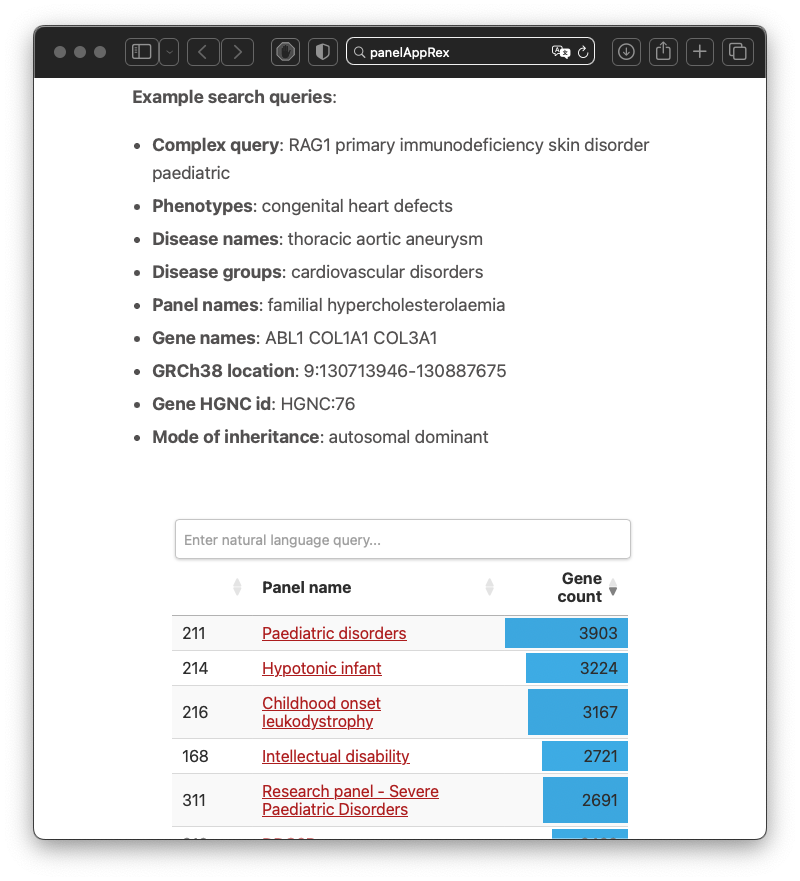
\includegraphics[width=0.49\textwidth]{screenshot_1.png}
    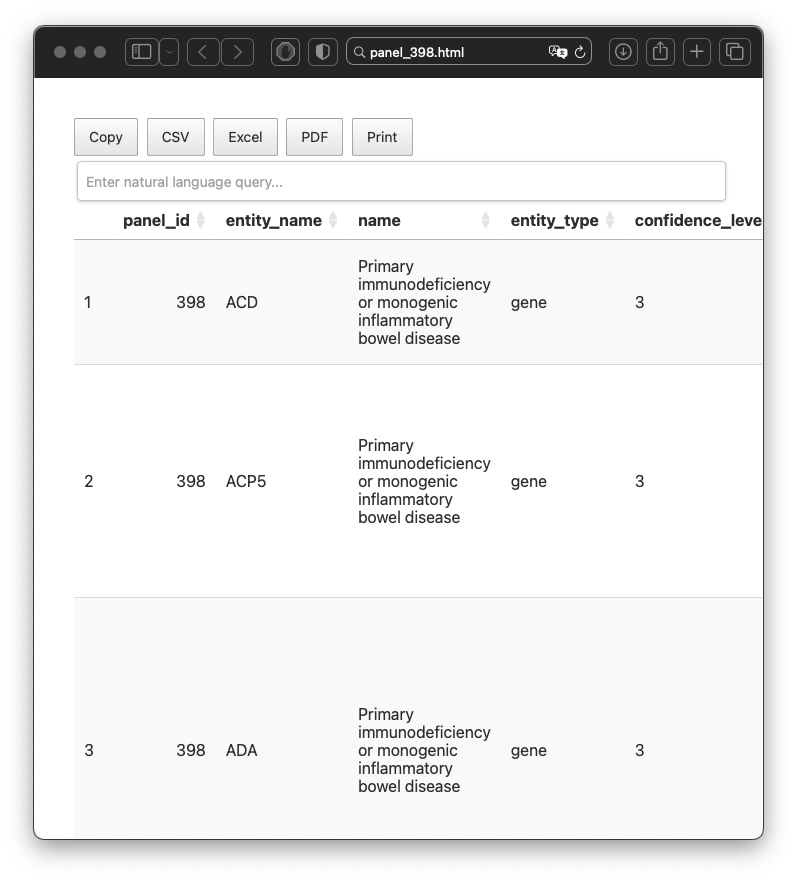
\includegraphics[width=0.49\textwidth]{screenshot_2.png}    
    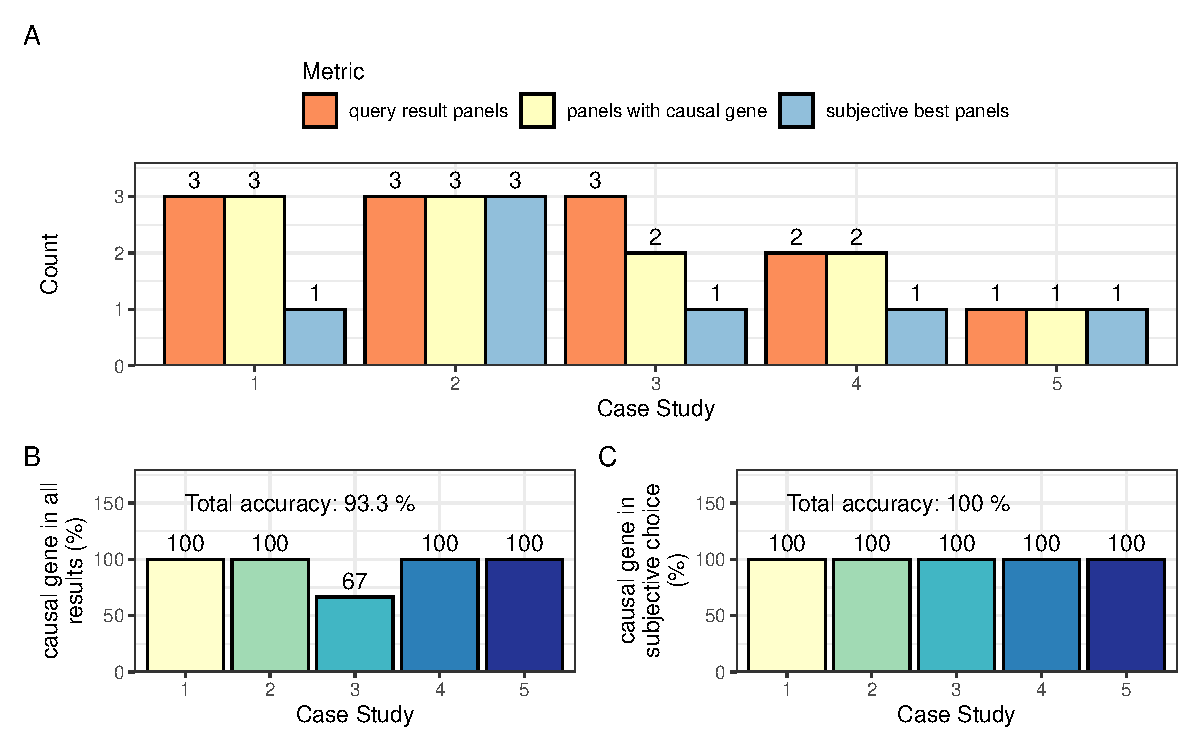
\includegraphics[width=0.85\textwidth]{benchmark.pdf}    
 %  \caption{PanelAppRex interface displaying search results for a complex natural language query. The top panels show screenshots: the left displays the full database before filtering, and the right shows detailed results for a selected panel. Below, benchmark metrics are presented: (A) the number of panels queried per case study, (B) the percentage of panels that included the true causal gene, and (C) the percentage from the single best panel selection that contained the true causal gene.}

\caption{PanelAppRex interface displaying search results for a complex query. Top: screenshots showing the search interface, with the left panel displaying the full database before filtering and the right panel showing detailed results for a selected panel. Bottom: benchmark metrics are presented as follows: (A) for each of the 5 case studies, the total number of panels returned, the number of panels that included the causal gene, and the single best panel selected (always 1 by default); (B) the percentage of all returned panels that included the true causal gene; (C) the percentage of the single best panels that contained the true causal gene.}


    \label{fig:performance}
\end{figure}

\subsection{Validation benchmarking}
\noindent
To mimic a clinician diagnosing a new disease such as \ac{pid}, we began by systematically selecting genetic diagnosis case studies from the current online catalogue from the \ac{jaci}, using the first five results  \cite{arruda_genetic_2015, 
mcaleer_severe_2015,
verhoeven_hematopoietic_2022,
magerus-chatinet_autoimmune_2013,
sharfe_fatal_2014}. We chose this source because our research centres on the genetic diagnosis of \ac{pid}.
The clinical background from these studies was used to construct keyword queries from patient features, simulating a naïve starting position for a clinician (full sources, queries, and results in \textbf{supplemental table 1}). We then tested whether our PanelAppRex tool could successfully retrieve panels that included the final causal gene reported in each case study. 

The tool's query process retrieves gene panels using natural language-style input. For example, in the first case study on Hereditary Angioedema, the clinician reported suspecting that the condition was linked to ``\textit{SERPING1}, Factor XII, and edema" which we used as the query terms. Although the true causal gene, \textit{F12}, was not mentioned, the inclusion of the related disease terms enabled the system to correctly retrieve the panel containing \textit{F12} based on the hidden search knowledge.

In our evaluation, PanelAppRex returned panels in which the causal gene was present in 93\% of all returned panels, with the user-selected best panel achieving a perfect accuracy of 100\% 
(\textbf{Figure \ref{fig:performance}}).
 These metrics were derived by comparing the causal gene identified from the case study abstracts to the panels returned by our query, and by applying a subjective relevance measure to mimic intuitive panel selection - acknowledging that certain panels, such as the established PID gene panel, are inherently more reliable than broader, less specific panels. Overall, the results confirm that our approach accurately identifies the most relevant panels and effectively supports clinical decision-making in complex diagnostic scenarios.

\FloatBarrier
\section{Summary}
\noindent
PanelAppRex offers a robust solution for aggregating and querying gene panel data. Its sophisticated search feature simplifies data exploration and enhances variant interpretation. Future work will focus on expanding the range of supported queries and integrating additional genomic data sources, further supporting the needs of clinicians and researchers.

\section*{Acknowledgements}
\noindent
We acknowledge \ac{ge} for providing public access to the PanelApp data.
The use of data from \ac{ge} panelapp was licensed under the Apache License 2.0.
The use of data from UniProt was licensed under Creative Commons Attribution 4.0 International (CC BY 4.0).
ClinVar asks its users who distribute or copy data to provide attribution to them as a data source in publications and websites \cite{landrum_clinvar_2018}.

\section*{Competing interest}
\noindent
We declare no competing interest. 

\bibliographystyle{unsrtnat}
\bibliography{references.bib}
\clearpage

\end{document}